\section{Evaluation}
\label{sec:evaluation}

In this section we present a quantitative evaluation \textit{for two corpus} of the algorithm proposed in this paper \textit{and a comparative evaluation}. In the GRE area there was a common assumption that there is a gold standard ordering for a given domain~\cite{Dale1995}. However, this assumption has been dropped after empirical studies such as those presented in~\cite{arec2:2008:Areces,viet:gene11}. It has been observed that not only there is no single ordering of properties that covers all human-produced descriptions in a given domain but, in fact, it is not even the case that each speaker consistently uses just one ordering. In this section we show that the probabilistic algorithm presented in the previous section is able to generate a distribution of REs similar to that observed in corpora, even when no corpus specific for a target object is available. 


%\subsection{Evaluation of the GRE3D7}
%\label{sec:evaluacionGRE3D7}

\textit{A quantitative evaluation over the GRE3D7}. Using \puse learned as described in Section~\ref{sec:learning} and running our algorithm 10000 times, we obtain 14 different referring expressions for Figure~\ref{GRE3D7-stimulus}. The algorithm generates 5 of the 12 different kinds of REs observed in the 140 occurrences of the corpora. We also generate other 9 REs for the target, not present in the corpora, but natural sounding as can be observed in Table~\ref{results-algo-fig3} that only represent a 1,52\% of the utterances generated by the algorithm. Hence, 98,48\% of the utterances generated by the algorithm appear in the corpora. In the table we list all the REs found in the corpus for Figure~\ref{GRE3D7-stimulus} and all the RE generated by our algorithm using the learned \puse. For each RE, we indicate the number of times it appears in the corpus (\#Cor), the proportion of the corpus its frequency represents (\%Cor), the number of times it is generated by our algorithm (\#Alg) and the proportion of the generated REs its frequency represents (\%Alg). Finally, the accuracy (\%Acc) column compares the REs in the corpus with respect to the REs generated by the algorithm. The accuracy is the proportion of perfect matches between the algorithm output and the human REs from the corpus. The accuracy metric has been used in previous work for comparing the output of a REG algorithm with the REs found in corpora~\cite{sluis07:eval,viet:gene11} and is considered an strict comparison metric for this task. 

\begin{table}[h!]
\begin{center}
\begin{tabular}{|l|c|c|c|c|c|}
\hline
RE & \#Cor & \%Cor & \#Alg & \%Alg & \%Acc \\
\hline
ball,green & 91 & 65 & 6376 & 63,76 & 63,76 \\
ball,green,small & 23 & 16,43 & 3440 & 34,40 & 16,43 \\
ball,green,small,on-top(blue,cube,large) & 8 & 5,71 & 0 & 0 & 0 \\
ball,green,on-top(blue,cube) & 5 & 3,57 & 0 & 0 & 0 \\
ball,green,on-top(blue,cube,large) & 5 & 3,57 & 0 & 0 & 0 \\
ball,green,small,on-top(blue,cube) & 2 & 1,43 & 0 & 0 & 0 \\
ball,on-top(cube) & 1 & 0,71 & 27 & 0,27 & 0,27 \\
ball,green,small,on-top(blue,cube,large,left) & 1 & 0,71 & 0 & 0 & 0 \\
ball,small,on-top(cube,large)	& 1 & 0,71 & 2 & 0,02 & 0,02 \\
ball,green,top & 1 & 0,71 &	0 & 0 & 0 \\
ball,small,on-top(cube) & 1 & 0,71 & 3 & 0,03 & 0,03 \\
ball,green,on-top(cube) & 1 & 0,71 & 0 & 0 & 0 \\
ball,front,green & 0 & 0 & 97 & 0,97 & 0 \\
ball,front,green,small & 0 & 0 & 13 & 0,13 & 0 \\
ball,front,top & 0 & 0 & 12 & 0,12 & 0 \\
ball,green,left	& 0 & 0 & 11 & 0,11 & 0 \\
%ball,on-top(blue,cube) & 0 & 0 & 32 & 0,32 & 0 \\
ball,top & 0 & 0 & 10 & 0,10 & 0 \\
ball,green,left,small & 0 & 0 & 5 & 0,05 & 0 \\
ball,left,top & 0 & 0 & 2 & 0,02 & 0 \\
ball,small,top & 0 & 0 & 1 & 0,01 & 0 \\
ball,front,on-top(cube,left) & 0 & 0 & 1 & 0,01 & 0 \\
%ball,green,small,on-top & 0 & 0 & 14 & 0,14 & 0 \\
%ball,green,left,on-top(blue,cube),small & 0 &  0 & 7 & 0,07 & 0 \\
\hline
Total & 140 & 100 & 10000 & 100 & 80,51 \\
\hline
\end{tabular}
\caption{Referring expressions produced by the algorithm for Figure~\ref{GRE3D7-stimulus}\label{results-algo-fig3}}
\end{center}
\end{table}

In order to put our results in perspective we compare the accuracy obtained for \textit{all} figures in the corpus using the probability of used inferred (column Learned \puse) and the probability of used directly extracted from corpora (column Model \puse) as explained in Section~\ref{sec:learning}. We show the accuracy results in Table~\ref{results-algo-all}. The random baseline (column Random) is calculated in by producing random probabilities of use and then running the algorithm 10000 using these random probabilities. Not only the intersection between the randomly generated REs and the corpus is lower but also many of  the REs generated in this way are not naturally sounding (e.g. ``small on the top of a blue cube that is below of something that is small''). We also show the results of accuracy for uniform distribution (column Uniform) as a second baseline. We calculate the uniform distribution by assigning each RE generated by the algorithm or in corpora the same proportion. 

\begin{table}[h!]
\begin{center}
\begin{tabular}{|l|c|c|c|c|}
\hline
Figure & Model \puse &  Learning \puse & Random \puse &  Uniform \puse \\
\hline

Fig. 1	&	89,29\%	&	85,62\%	&	24,75\%	&	0.00\\%	\\
Fig. 2	&	73,28\%	&	63,66\%	&	6,99\%	&	0.00\\%	\\
Fig. 3	&	82,93\%	&	81,53\%	&	3,61\%	&	0.00\\%	\\
Fig. 4	&	69,41\%	&	73,73\%	&	1,37\%	&	0.00\\%	\\
Fig. 5	&	90,65\%	&	51,59\%	&	0,13\%	&	0.00\\%	\\
Fig. 6	&	87,24\%	&	80,35\%	&	4,35\%	&	0.00\\%	\\
Fig. 7	&	84,25\%	&	51,26\%	&	5,19\%	&	0.00\\%	\\
Fig. 8	&	80,94\%	&	72,92\%	&	4,39\%	&	0.00\\%	\\
Fig. 9	&	90,89\%	&	70,33\%	&	0,87\%	&	0.00\\%	\\
Fig. 10	&	91,31\%	&	73,96\%	&	8,75\%	&	0.00\\%	\\
Fig. 11	&	80,64\%	&	58,76\%	&	0,36\%	&	0.00\\%	\\
Fig. 12	&	77,16\%	&	76,06\%	&	0,2\%	&	0.00\\%	\\
Fig. 13	&	91,18\%	&	49,87\%	&	1,44\%	&	0.00\\%	\\
Fig. 14	&	94,44\%	&	68,7\%	&	1,35\%	&	0.00\\%	\\
Fig. 15	&	85,07\%	&	46,49\%	&	3,14\%	&	0.00\\%	\\
Fig. 16	&	82,4\%	&	61,79\%	&	0,52\%	&	0.00\\%	\\
Fig. 17	&	92,65\%	&	86,59\%	&	6,92\%	&	0.00\\%	\\
Fig. 18	&	90,24\%	&	77,34\%	&	31,66\%	&	0.00\\%	\\
Fig. 19	&	90,83\%	&	78,73\%	&	0,2\%	&	0.00\\%	\\
Fig. 20	&	83,65\%	&	67,48\%	&	1,79\%	&	0.00\\%	\\
Fig. 21	&	92,81\%	&	83,47\%	&	2,77\%	&	0.00\\%	\\
Fig. 22	&	88,34\%	&	83,05\%	&	1,56\%	&	0.00\\%	\\
Fig. 23	&	85,92\%	&	71,11\%	&	0,73\%	&	0.00\\%	\\
Fig. 24	&	89,86\%	&	79,37\%	&	1,98\%	&	0.00\\%	\\
Fig. 25	&	86,33\%	&	70,05\%	&	11,97\%	&	0.00\\%	\\
Fig. 26	&	86,52\%	&	71,98\%	&	15,58\%	&	0.00\\%	\\
Fig. 27	&	71,59\%	&	67,78\%	&	2,79\%	&	0.00\\%	\\
Fig. 28	&	78,4\%	&	77,13\%	&	1,6\%	&	0.00\\%	\\
Fig. 29	&	92,36\%	&	73,83\%	&	1,78\%	&	0.00\\%	\\
Fig. 30	&	89,64\%	&	70,41\%	&	38,83\%	&	0.00\\%	\\
Fig. 31	&	85,85\%	&	70,98\%	&	0,88\%	&	0.00\\%	\\
Fig. 32	&	86,46\%	&	73,11\%	&	5,68\%	&	0.00\\%	\\
\hline
Average	&	85.7\%	&	70.91\%	&	6.07\%	&	0.00\%	\\

\hline
\end{tabular}
\caption{Percentage on intersection between the REs generated using directly extracted from the figure corpora\label{results-algo-all}, learned probabilities, random and uniform probabilities}
\end{center}
\end{table}

The table shows that the accuracy is not stable for all scenes, ranging from 86.59\% in Fig. 17 to 46.49\% in Fig. 15. The drop in accuracy that we see for Fig 15 is due to the characteristic of the behavior of size in the domain that we were not able to capture and that we discussed in Section~\ref{sec:learning}. 

%\subsection{Evaluation of the TUNA-corpus}
%\label{sec:evaluationTUNA}

\textit{A comparative evaluation for the TUNA-corpus. 
Using \puse learned as described in Section~\ref{sec:learning} and running our algorithm 100 times we adquire the following results:
About the evaluation method 
In the evaluation results reported below, we use the intrinsic methods used in the ASGRE Challenge. Minimality, defined as the proportion of descriptions produced by a system
that are maximally brief, as per the original definition in Dale (1989). The Dice coefficient, used to compare the description produced by
a system to the human-produced description on the same input domain. %Dice is estimated
%as follows:
%2 × |DS ∩ DH |
%|DS | + |DH |
MASI, a version of the Jaccard similarity coefficient proposed
by Passonneau (2006) which multiplies the similarity value by a monotonicity coefficient, biasing
the measure towards those cases where DS and
DH have an empty set difference. Intuitively, this
means that those system-produced descriptions are
preferred which do not include attributes that are
omitted by a human. Thus, two of our intrinsic measures assess Humanlikeness (Dice and MASI), while
Minimality reflects the extent to which an algorithm
conforms to brevity, one of the principles that has
emerged from the ASGRE literature.}

\begin{table}[h!]
\begin{center}
\begin{tabular}{|l|c|c|c|c|c|}
\hline
%Figure & Model \puse &  Learning \puse & Random \puse &  Uniform \puse \\
	& DICE	&	MASI	&	A\_ACCURACY	&	UNIQUENESS	&	MINIMALITY	\\
\hline
Furniture	&	0,79\%	&	0,58\%	&	0,43\%	&	0,48\%	&	0,0125\%	\\
People	&	0,65\%	&	0,37\%	&	0,19\%	&	1\%	&	0,0\%	\\
\hline
\end{tabular}
\caption{Percentage average adquired for Furniture and People}
\end{center}
\end{table}


\textit{We also did another comparison taking into account the 20 first RE that the system produced, and when in those 20 is the given for a human we choise this one, we obtain the following results:}

\begin{table}[h!]
\begin{center}
\begin{tabular}{|l|c|c|c|c|c|}
\hline
%Figure & Model \puse &  Learning \puse & Random \puse &  Uniform \puse \\
&	DICE	&	MASI	&	A\_ACCURACY	&	UNIQUENESS	&	MINIMALITY	\\
\hline
Furniture	&	0,87\%	&	0,7525\%	&	0,65\%	&	0,4625\%	&	0,0125\%	\\
People	&	0,81\%	&	0,68\%	&	0,60\%	&	0,97\%	&	0,0147\%	\\
\hline
\end{tabular}
\caption{Percentage average adquired for Furniture and People considering 20 first frequencies}
\end{center}
\end{table}


\textit{We compare our results with the algorithm that win the ASGRE-challenge in 2008, we used the same corpus and the same tools provided for the organization of the challenge, we will show DICE, MASI, A\_ACCURACY, UNIQUENESS and MINIMALITY. \cite{graph08}}

\begin{figure}[h!]
\begin{center}
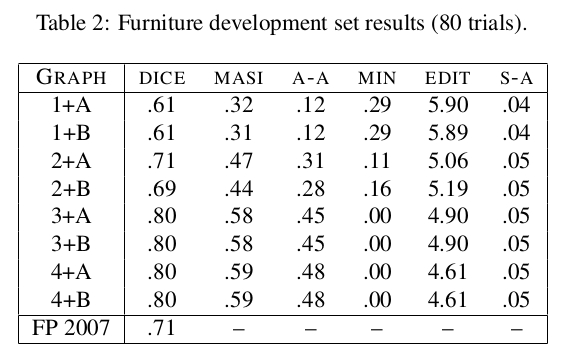
\includegraphics[width=.7\textwidth]{images/graphResults.jpg}
\end{center}
\vspace*{-2em}
\caption{Graph results \label{graphResults}}
\end{figure}

\begin{figure}[h!]
\begin{center}
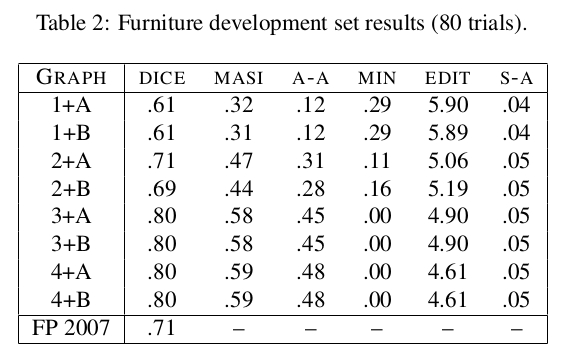
\includegraphics[width=.7\textwidth]{images/graphResults.jpg}
\end{center}
\vspace*{-2em}
\caption{Graph results \label{graphResults2}}
\end{figure}

\textit{They have severals systems that take into account a costs functions 4 kind of systems: 1 Simple, 2 Stochastic, 3 Free-stochastic, 4 Free-naive and for each those the Orders A Random and B Cost-based. The system submitted to the challenge was the 4 B.}\\

\textit{Our results taking in count the first one RE produced by thes system is comparable to their results, but with a lower measures, if we take into account our the results allowing more than just one RE, our results are better.}

To show the results from a different perspective than that of accuracy we also compute the cross-entropy~\cite{juraksky:spee08} between the corpus distribution of REs and each algorithm (the Model, the Learned, and the two baselines).    

%The entropy a measure of the amount of uncertainty associated with the value of the variable. The cross entropy between two probability distributions measures the average number of bits needed to identify an event from a set of possibilities. The cross entropy for two distributions p and q over the same probability space can be calculate by the formula... 
%chapter 6.7 

In Figure~\ref{Entropy} we show the results that we obtains for each scene in Table~\ref{results-algo-all} 
%\texit{over the GRE3D7.} 

\begin{figure}[h!]
\begin{center}
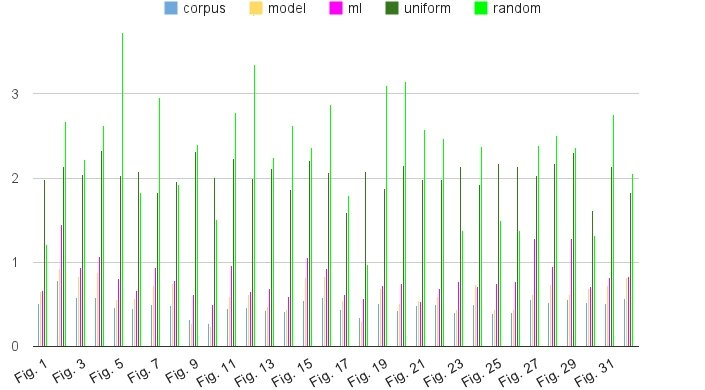
\includegraphics[width=.9\textwidth]{images/entropyComplete.jpg}
\end{center}
\vspace*{-2em}
\caption{Cross-entropy between the corpus distribution of REs and each algorithm} \textit{over the GRE3D7}\label{Entropy}
\end{figure}

In the figure we can observe that the learning and model cross-entropies are, in general, much closer to the corpus entropy than the random and uniform cross-entropies. \textit{In Figures 18 and 30 the random distribution are better and closer to learning and model because the randomly selected values of \puse are close to the learned values of \puse by chance. Those are also evident in Table~\ref{results-algo-all} where random are 31,66\% for Fig. 18 and 38,83\% for Fig. 30.}
In the figure we can also observe that the algorithm that uses the \puse directly calculated on the corpus of the scene (model) has a cross-entropy with respect to the corpus distribution that is very close to the cross-entropy between the corpus distribution and the distribution obtained by the algorithm when run with the \puse learned from corpora that does not describe the target scene (learning). This observation supports the learning mechanism proposed in Section~\ref{subsec:learning} to estimate the \puse when no corpora of REs of the target scene is available. 
